\section{Appendix Section}
\label{sec:appendix_section}

\subsection{Additional SDFusion fine-tuning results}
\label{sec:appendic_fine_tuning}

\iffalse
\begin{figure}[h]
  \centering
  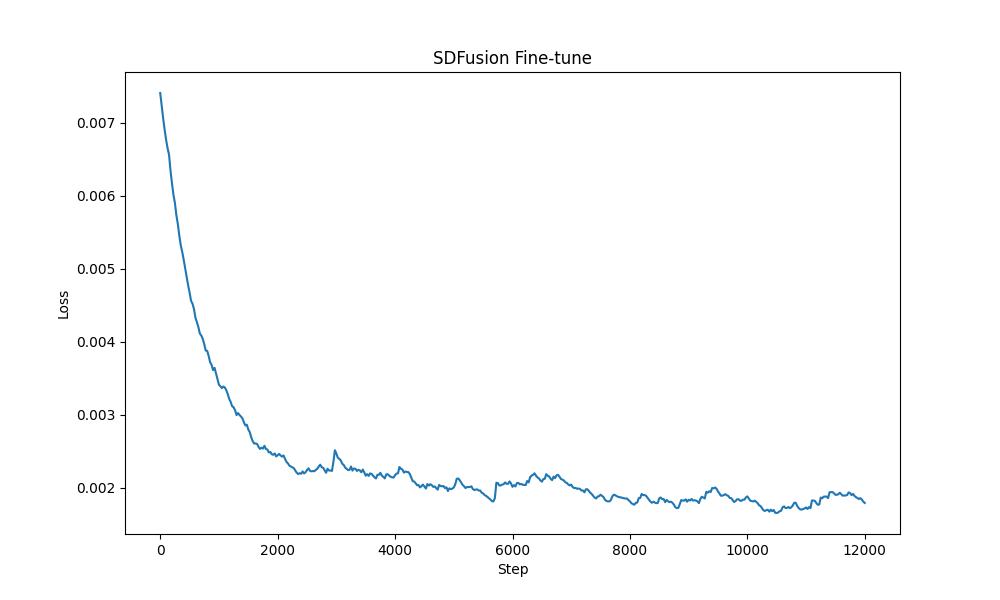
\includegraphics[width=\linewidth]{figs/sdfusion_finetune_loss_plot.png}
  \caption{Loss curve of our SDFusion fine-tune (smoothed).}
  \label{fig:finetune}
\end{figure}

\begin{figure}[h]
  \centering
  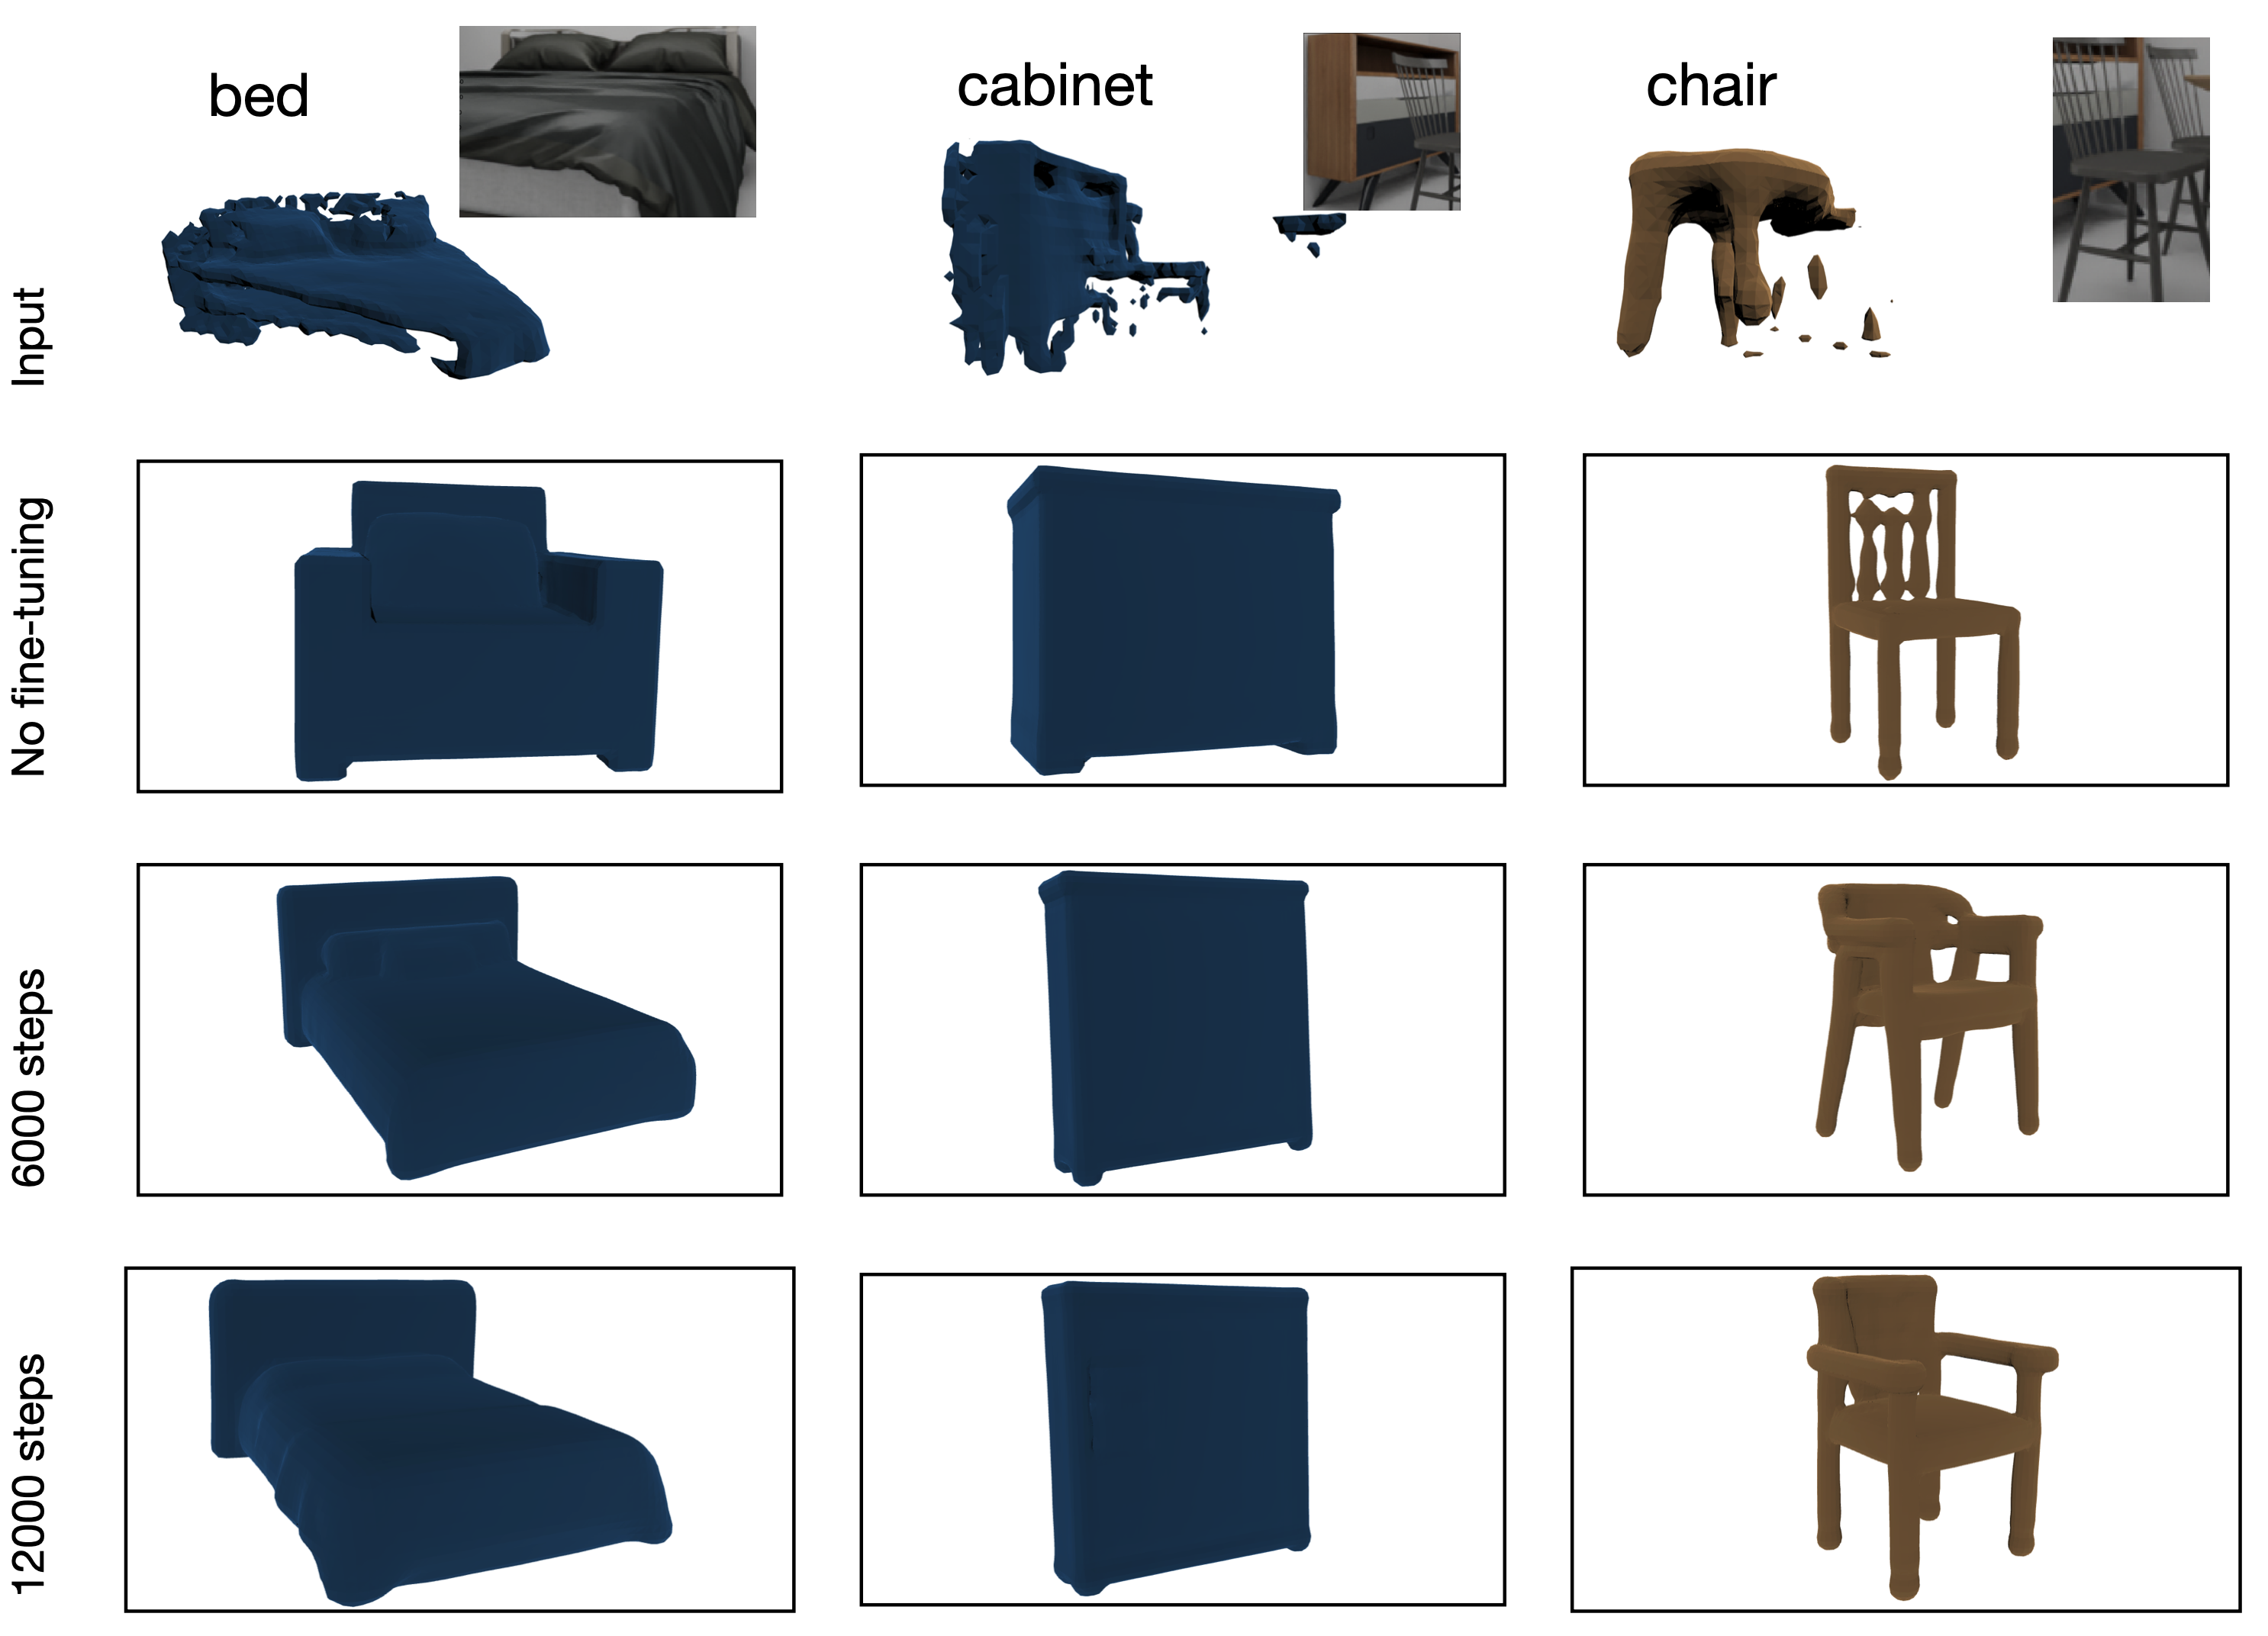
\includegraphics[width=80mm, scale=1]{images/image4.png}
  \caption{Fine-tuning results for SDFusion}
\end{figure}
\fi


\begin{figure}[h]
  \centering
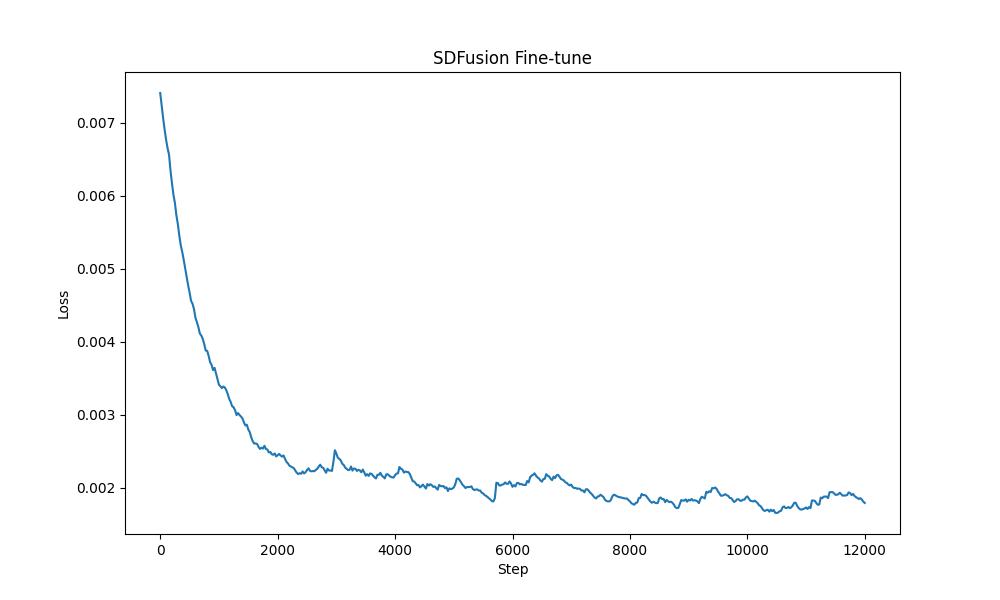
\includegraphics[width=\linewidth]{figs/sdfusion_finetune_loss_plot.png}
  \caption{Loss curve of our SDFusion fine-tune (smoothed).}
\label{fig:finetune}
\end{figure}

\begin{figure}[h]
  \centering
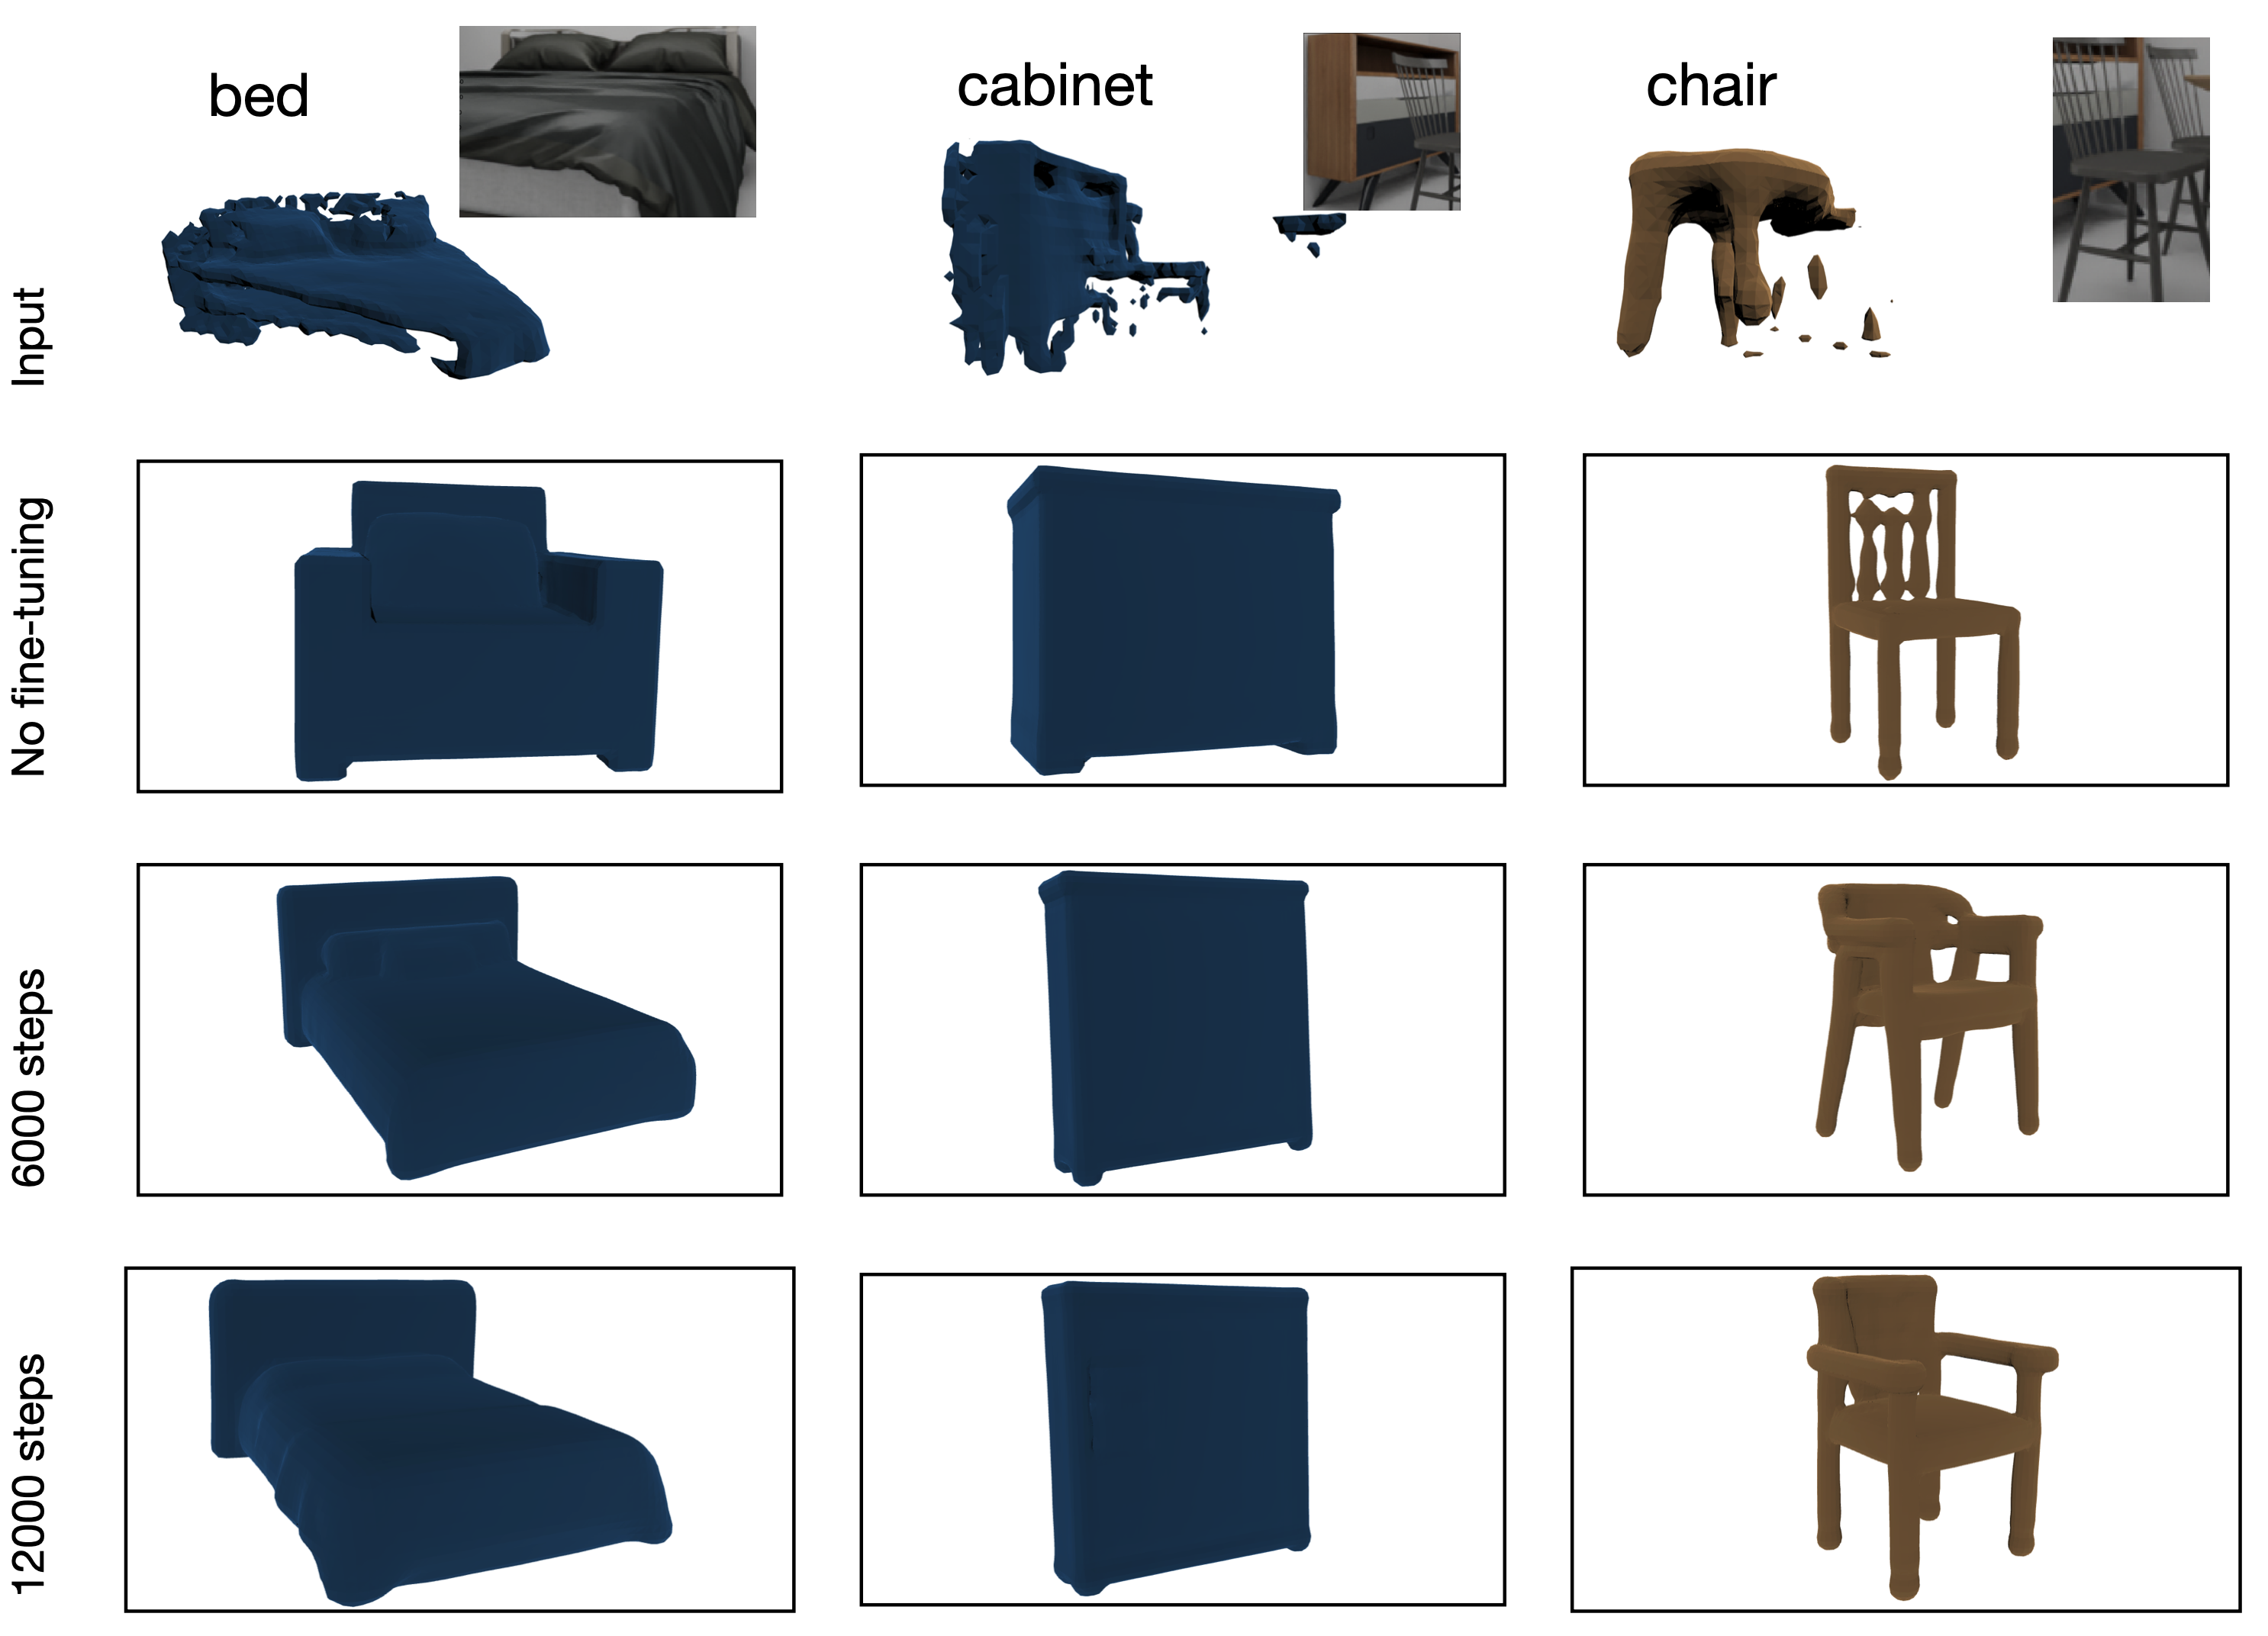
\includegraphics[width=\linewidth]{images/image4.png}
  \caption{Effect of fine-tuning SDFusion on reconstruction results. The process of fine-tuning significantly enhances our capacity to generate objects that more accurately align with those presented in Front3D. A notable improvement is observed in the refined geometries of beds. Prior to fine-tuning, the standard SDFusion model produced representations resembling armchairs; however, post-fine-tuning, the model successfully generates geometries that appropriately resemble beds.}
  \label{fig:short-b}
\end{figure}

The loss curve in \cref{fig:finetune} shows that the fine-tuning process was successful. The results of the fine-tuning process are shown in \cref{fig:short-b}.
We used the conversion procedure from \citet{cheng2023sdfusion} to convert the object meshes from the dataset to signed distance fields.
We train the model for 12,000 steps using the original hyperparameters from \citet{cheng2023sdfusion} but with a batch size of 32.
The dataset contains 16,000 samples, hence the 12,000 steps of fine-tuning correspond to 24 epochs with a batch size of 32.

\newpage

\subsection{Additional Panoptic 3D retraining results}

% \begin{figure*}
%   \centering
%   \begin{minipage}{0.49\linewidth}
%     \centering
%   \begin{subfigure}[b]{0.45\linewidth}
%     \centering
%     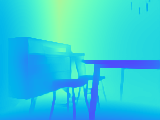
\includegraphics[width=\linewidth]{figs/depth_ours.png}
%     \label{subfig:sub1}
%    \vspace*{-3mm} % Adjust vertical spacing between the caption and the images
%   \caption{Depth map (ours).}
%   \end{subfigure}
%   \hfill
%   \begin{subfigure}[b]{0.45\linewidth}
%     \centering
%     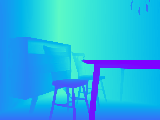
\includegraphics[width=\linewidth]{figs/depth_pan.png}
%     \label{subfig:sub2}
%    \vspace*{-3mm} % Adjust vertical spacing between the caption and the images
%   \caption{Depth map (\citep{dahnert2021panoptic}).}
%   \end{subfigure}

%   \vspace{0.03\linewidth} % Adjust vertical spacing between rows of figures

%   \begin{subfigure}[b]{0.45\linewidth}
%     \centering
%     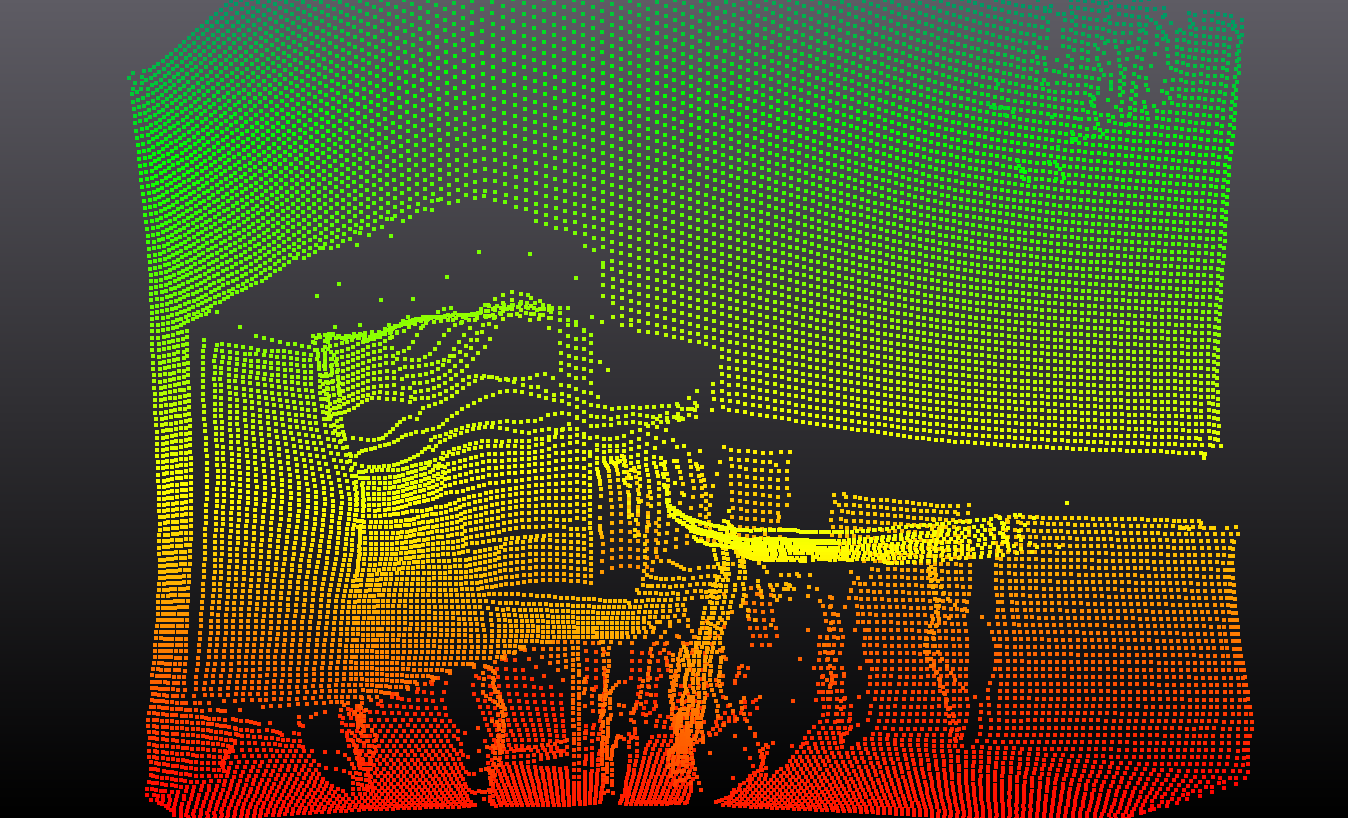
\includegraphics[width=\linewidth]{figs/depthply_ours.png}
%     \label{subfig:sub3}
%    \vspace*{-3mm} % Adjust vertical spacing between the caption and the images
%    \caption{Geometry from depth (ours).}
%   \end{subfigure}
%   \hfill
%   \begin{subfigure}[b]{0.45\linewidth}
%     \centering
%     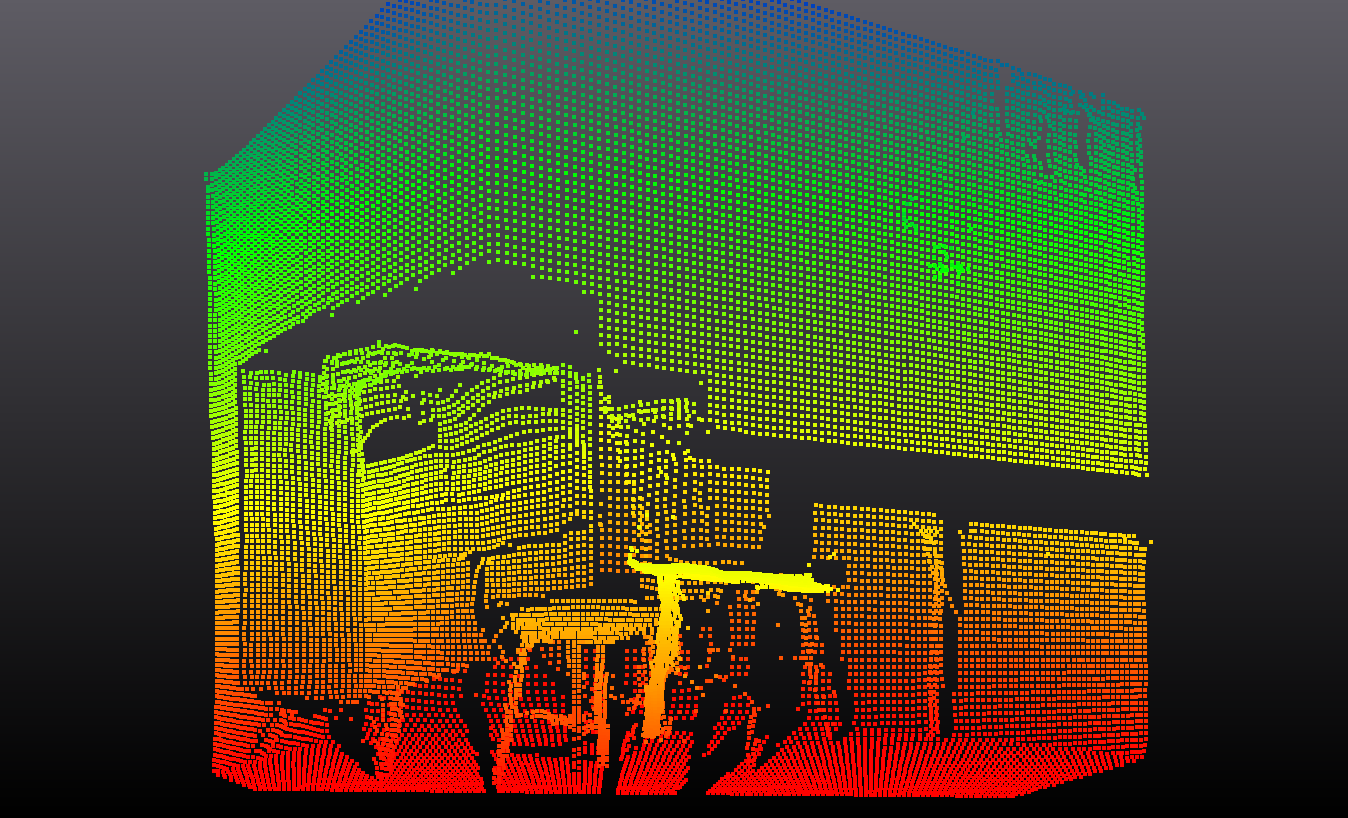
\includegraphics[width=\linewidth]{figs/depthply_pan.png}
%     \label{subfig:sub4}
%    \vspace*{-3mm} % Adjust vertical spacing between the caption and the images
%    \caption{Geometry from depth (\citep{dahnert2021panoptic}).}
%   \end{subfigure}

%   \caption{2D results from the Panoptic 3D model. Our re-training results (left) vs. results from \citet{dahnert2021panoptic} (right).}
%   \label{fig:qual_panoptic}
%   \end{minipage}
%   \hfill
%   \begin{minipage}{0.49\linewidth}
%     \centering
%     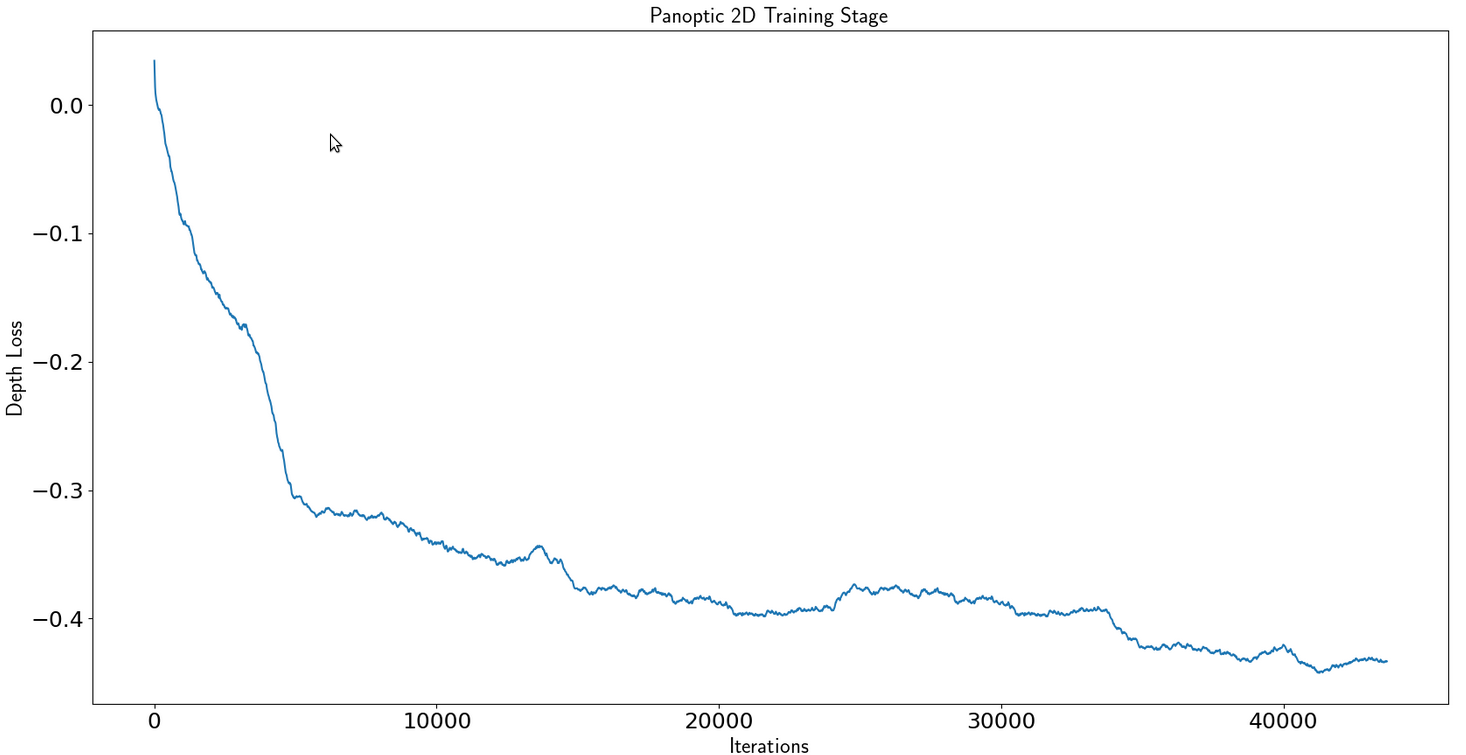
\includegraphics[width=\linewidth]{figs/depthloss.png}
%     \caption{Your caption for the additional figure.}
%     \label{subfig:additional}
%     \vspace*{-3mm} %
%   \end{minipage}
% \end{figure*}


\begin{figure}[h]
  \centering
  \begin{subfigure}[b]{0.45\linewidth}
    \centering
    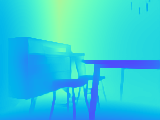
\includegraphics[width=\linewidth]{figs/depth_ours.png}
    \label{subfig:sub1}
   \vspace*{-3mm} % Adjust vertical spacing between the caption and the images
  \caption{Depth map (ours).}
  \end{subfigure}
  \hfill
  \begin{subfigure}[b]{0.45\linewidth}
    \centering
    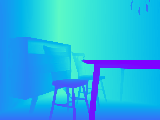
\includegraphics[width=\linewidth]{figs/depth_pan.png}
    \label{subfig:sub2}
   \vspace*{-3mm} % Adjust vertical spacing between the caption and the images
  \caption{Depth map (\citep{dahnert2021panoptic}).}
  \end{subfigure}

  \vspace{0.03\linewidth} % Adjust vertical spacing between rows of figures

  \begin{subfigure}[b]{0.45\linewidth}
    \centering
    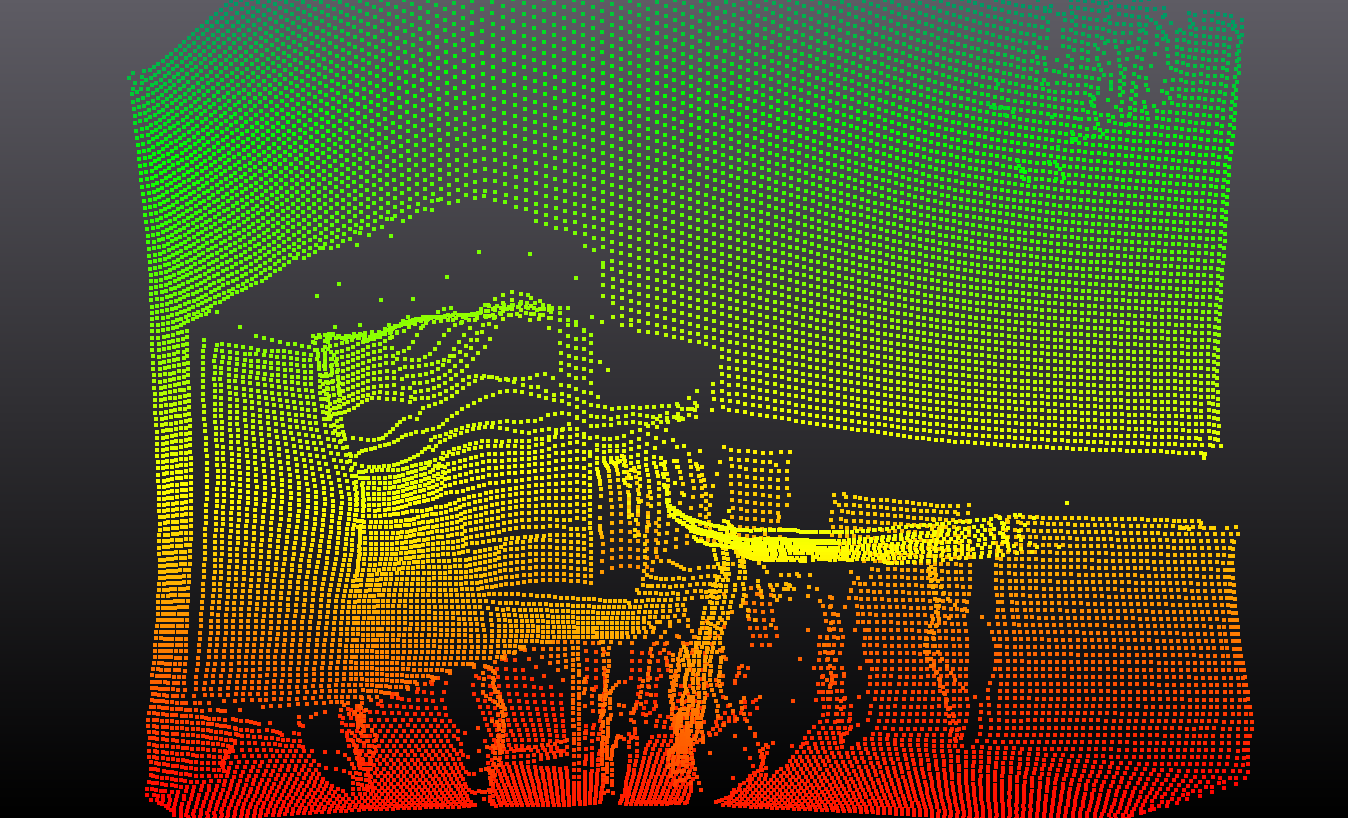
\includegraphics[width=\linewidth]{figs/depthply_ours.png}
    \label{subfig:sub3}
   \vspace*{-3mm} % Adjust vertical spacing between the caption and the images
   \caption{Geometry from depth (ours).}
  \end{subfigure}
  \hfill
  \begin{subfigure}[b]{0.45\linewidth}
    \centering
    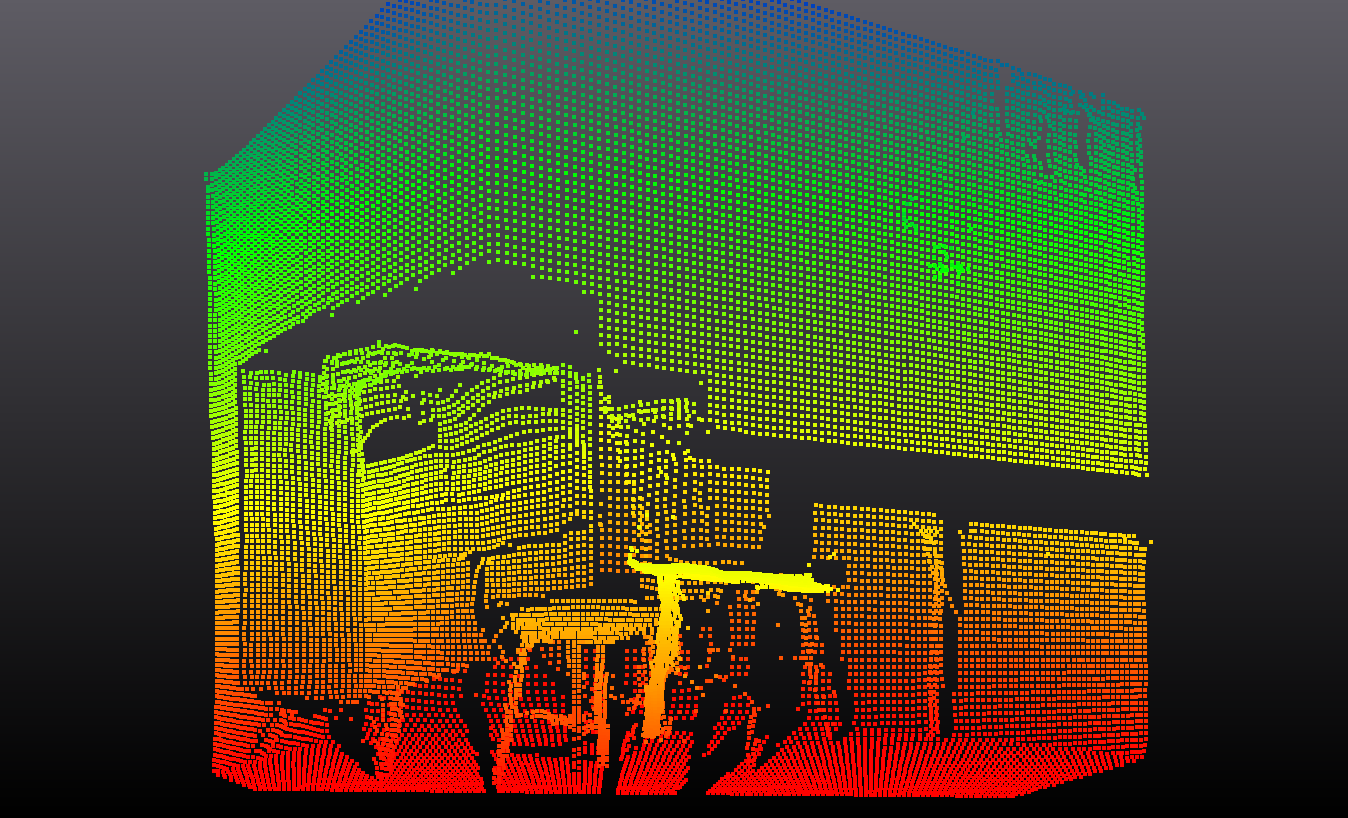
\includegraphics[width=\linewidth]{figs/depthply_pan.png}
    \label{subfig:sub4}
   \vspace*{-3mm} % Adjust vertical spacing between the caption and the images
   \caption{Geometry from depth (\citep{dahnert2021panoptic}).}
  \end{subfigure}

  \caption{2D results from the Panoptic 3D model. Our re-training results (left) vs. results from \citet{dahnert2021panoptic} (right).}
  \label{fig:qual_panoptic}
\end{figure}

\begin{figure}[h]
  \centering
  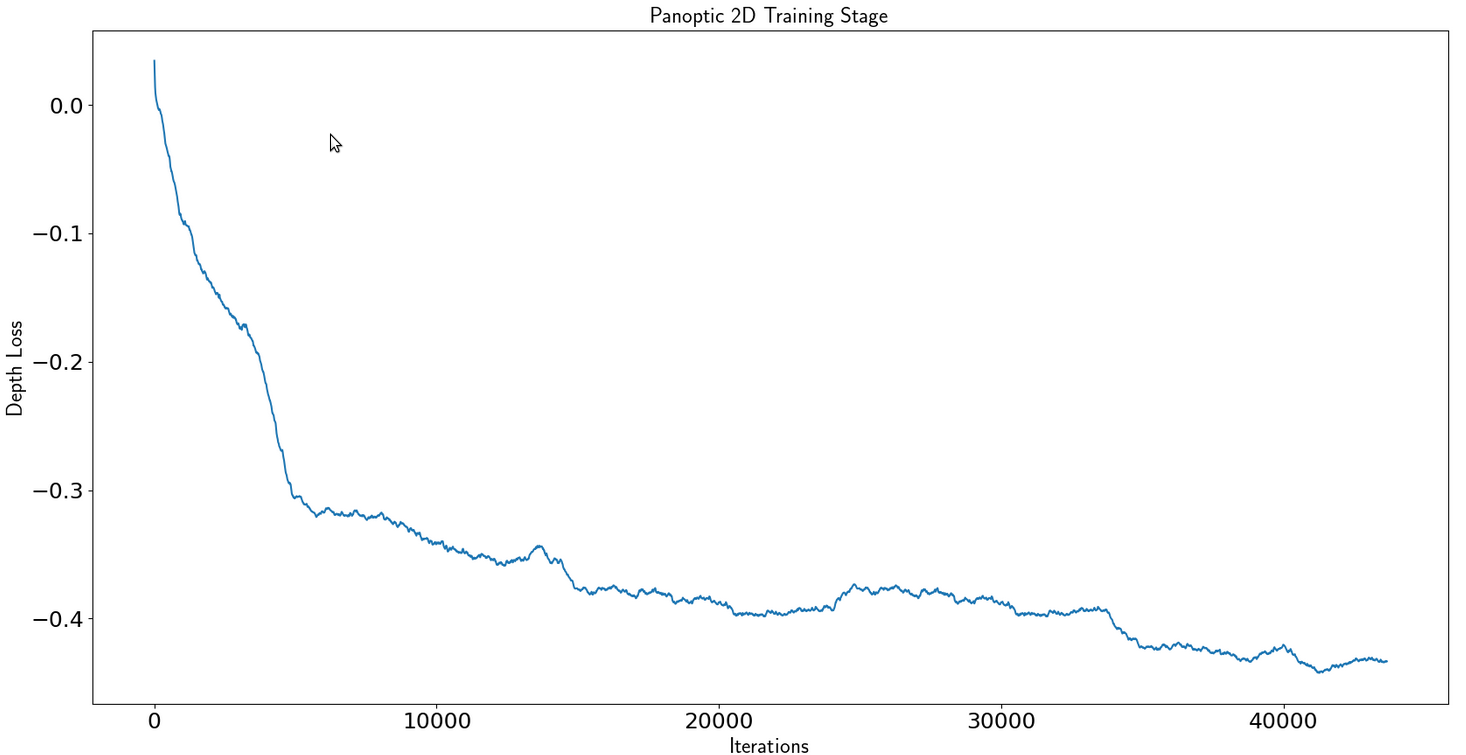
\includegraphics[width=\linewidth]{figs/depthloss.png}
  \caption{Depth loss curve for retraining of panoptic model (First 45k iterations).}
  \label{subfig:additional}
  \vspace*{-3mm} % Adjust vertical spacing between the caption and the image
\end{figure}

\subsection{Refined 3D scene inference details}
The results in \cref{sec:refinedrec} were generated using the pre-trained Panoptic 3D model and our fine-tuned version of SDFusion (6,000 steps checkpoint). 